%%%%%%%%%%%%%%%%%%%%%%%%%%%%%%%%%%%%%%%%%%%%%%%%%%%%%%%
%                   File: OSAmeetings.tex             %
%                  Date: 08 October 2018              %
%                                                     %
%     For preparing LaTeX manuscripts for submission  %
%       submission to OSA meetings and conferences    %
%                                                     %
%       (c) 2018 Optical Society of America           %
%%%%%%%%%%%%%%%%%%%%%%%%%%%%%%%%%%%%%%%%%%%%%%%%%%%%%%%

\documentclass[letterpaper,10pt]{article} 

%% if A4 paper needed, change letterpaper to A4

\usepackage{osameet3} %% use version 3 for proper copyright statement

\makeatletter
\renewcommand\@biblabel[1]{\fontsize{8}{9.6}\selectfont[#1]}
\renewenvironment{thebibliography}[1]
     {\section*{\refname
        \@mkboth{\MakeUppercase\refname}{\MakeUppercase\refname}}%
      \list{\@biblabel{\@arabic\c@enumiv}}%
           {\settowidth\labelwidth{\@biblabel{#1}}%
            \leftmargin\labelwidth
            \advance\leftmargin\labelsep
  \setlength{\parsep}{0pc}
  \setlength{\labelsep}{0.5em}
  \setlength{\itemsep}{0.05pc}
  \setlength{\listparindent}{0in}
  \setlength{\itemindent}{0in}
  \setlength{\rightmargin}{0in}
            \@openbib@code
            \usecounter{enumiv}%
            \let\p@enumiv\@empty
            \renewcommand\theenumiv{\@arabic\c@enumiv}}%
      \sloppy
      \clubpenalty4000
      \@clubpenalty \clubpenalty
      \widowpenalty4000%
      \sfcode`\.\@m\fontsize{8}{9.6}\selectfont}
     {\def\@noitemerr
       {\@latex@warning{Empty `thebibliography' environment}}%
      \endlist \vskip.2in}
\makeatother


%% standard packages and arguments should be modified as needed
\usepackage{amsmath,amssymb}
\usepackage[pdftex,colorlinks=true,bookmarks=false,citecolor=blue,urlcolor=blue]{hyperref} %pdflatex
%\usepackage[dvips,colorlinks=true,bookmarks=false,citecolor=blue,urlcolor=blue]{hyperref} %latex w/dvips
\usepackage[font=small]{caption}

\begin{document}

\title{FlexLION: A Reconfigurable All-to-All Optical Interconnect Fabric with Bandwidth Steering}
\vspace{-3ex}
\author{R. Proietti, G. Liu, X. Xiao, S. Werner, P. Fotouhi, S.J.B. Yoo}
\address{ Department of Electrical and Computer Engineering, University of California, Davis, CA 95616}
\email{rproietti@ucdavis.edu, sbyoo@ucdavis.edu}
\vspace{-3ex}

\begin{abstract}
We demonstrate an all-to-all interconnect fabric with bandwidth steering by wavelength routing, wavelength add/drop filtering and spatial switching. We report a proof-of-concept experiment and demonstrate scalability up to 32 ports with aggregated bandwidth of 51.2 Tb/s under worst-case crosstalk.

\end{abstract}

\ocis{(200.4650) Optical interconnects; (060.4265) Networks, wavelength routing}
\vspace{-3ex}
\section{Introduction}

Optical interconnects based on arrayed waveguide grating routers (AWGRs) \cite{AWGR_XT_1996} have attracted significant attention in optical networks on chips (NOCs), datacenter and high performance computing (HPC) applications thanks to AWGR’s ability to provide wavelength routing and all-to-all contentionless connectivity \cite{JLT2015_Proietti}. By exploiting wavelength division multiplexing (WDM) and wavelength routing property of AWGRs (see table in Fig. 1(a)), we can significantly reduce the complexity of an all-to-all topology. While all-to-all interconnection can assure single-hop communication between all the nodes in a network and represents an ideal interconnection topology for traffic patterns with uniform random behavior, communication patterns often exhibit uneven bandwidth requirements among different node pairs \cite{OSA_2014}. It would then be desirable to reconfigure the interconnection (as shown in Fig. 1(b)) to steer the bandwidth where needed (using either a traffic or application-driven approach) to better serve the communication demands. FlexLION (Flexible Low-latency Interconnect Optical Network) enables such reconfiguration by combining the all-to-all communication capability of an arrayed waveguide grating router (AWGR) with spatial switching (e.g. \cite{Han:15}) and wavelength add/drop filters (see Fig. 1(c)). Compared to our work in \cite{FlexECOC2018_Xian}, we significantly improved the bandwidth and wavelength reconfiguration granularity by introducing the use of add/drop tunable filters. We demonstrate FlexLION working principle using a 4-node testbed with off-the-shelf components, and assess the scalability up to 32 nodes under worst-case crosstalk scenario. 
\vspace{-2ex}
\begin{figure}[htbp]
  \centering
  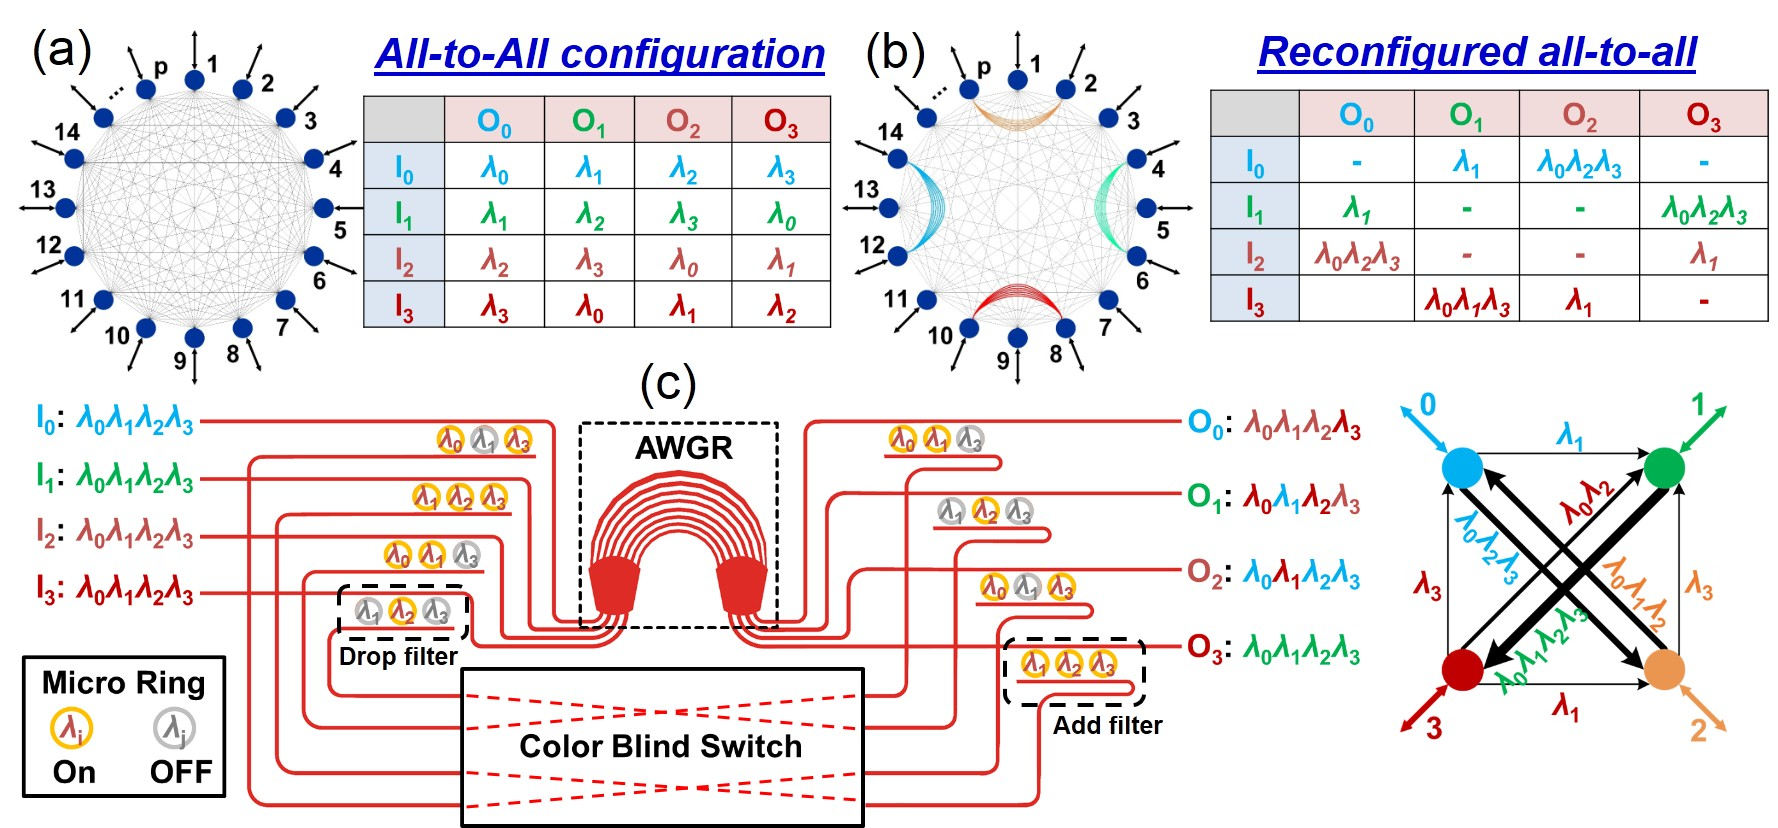
\includegraphics[width=15cm]{Figure1_v4.jpg}
\caption{(a) All-to-All interconnection among \textit{p} nodes and AWGR wavelength routing table for \textit{p}=4; (b) reconfigured all-to-all interconnection with bandwidth steering and example of FlexLION wavelength routing table after reconfiguration. (c) Four-node FlexLION architecture with AWGR, wavelength add/drop filters and color-blind optical switch. The routing table in (a) can be reconfigured as in (b) by tuning the wavelength add/drop filters (here represented with cascaded microring resonators) and setting up the spatial (color-blind) switch. This allows to steer and increase the bandwidth between node pairs 0,2 and 1,3.}
\vspace{-3ex}
\end{figure} 
\vspace{-3ex}

\section{Experimental Setup and Results}
Fig. 2(a) shows a FlexLION four-node testbed using four field programmable gate arrays (FPGAs) with 10 Gb/s WDM TRXs. Each FPGA connects to a 32-port 100 GHz spacing silica AWGR (used here as 4-port AWGR) through a pair of 1$\times$2 wavelength selective switches (WSSs). The WSSs on the left side are responsible to drop specific lambdas and send them to the color-blind switch (a 32-port Polatis switch in this setup). The WSSs on the right side are responsible for adding the lambdas switched by the color-blind switch and coupling them with the ones coming from the AWGR output ports. Fig. 2(b) shows the scenario implemented in the testbed before and after reconfiguration. Before reconfiguration, node4 receives only 10 Gb/s from node 1 at lambda 3. After reconfiguration, node4 receives 30 Gb/s from node1 by steering lambda 1 and lambda 2 (originally dedicated to node 2 and node 3) toward node 4. %we need to modify the diagram to add colors and lines to FIg. 2a and shows the dropped wavelengths
Fig.2(c) shows the BER values captured at Node 4 FPGA RXs before and after reconfiguration. 
\vspace{-2ex}
\begin{figure}[htbp]
  \centering
  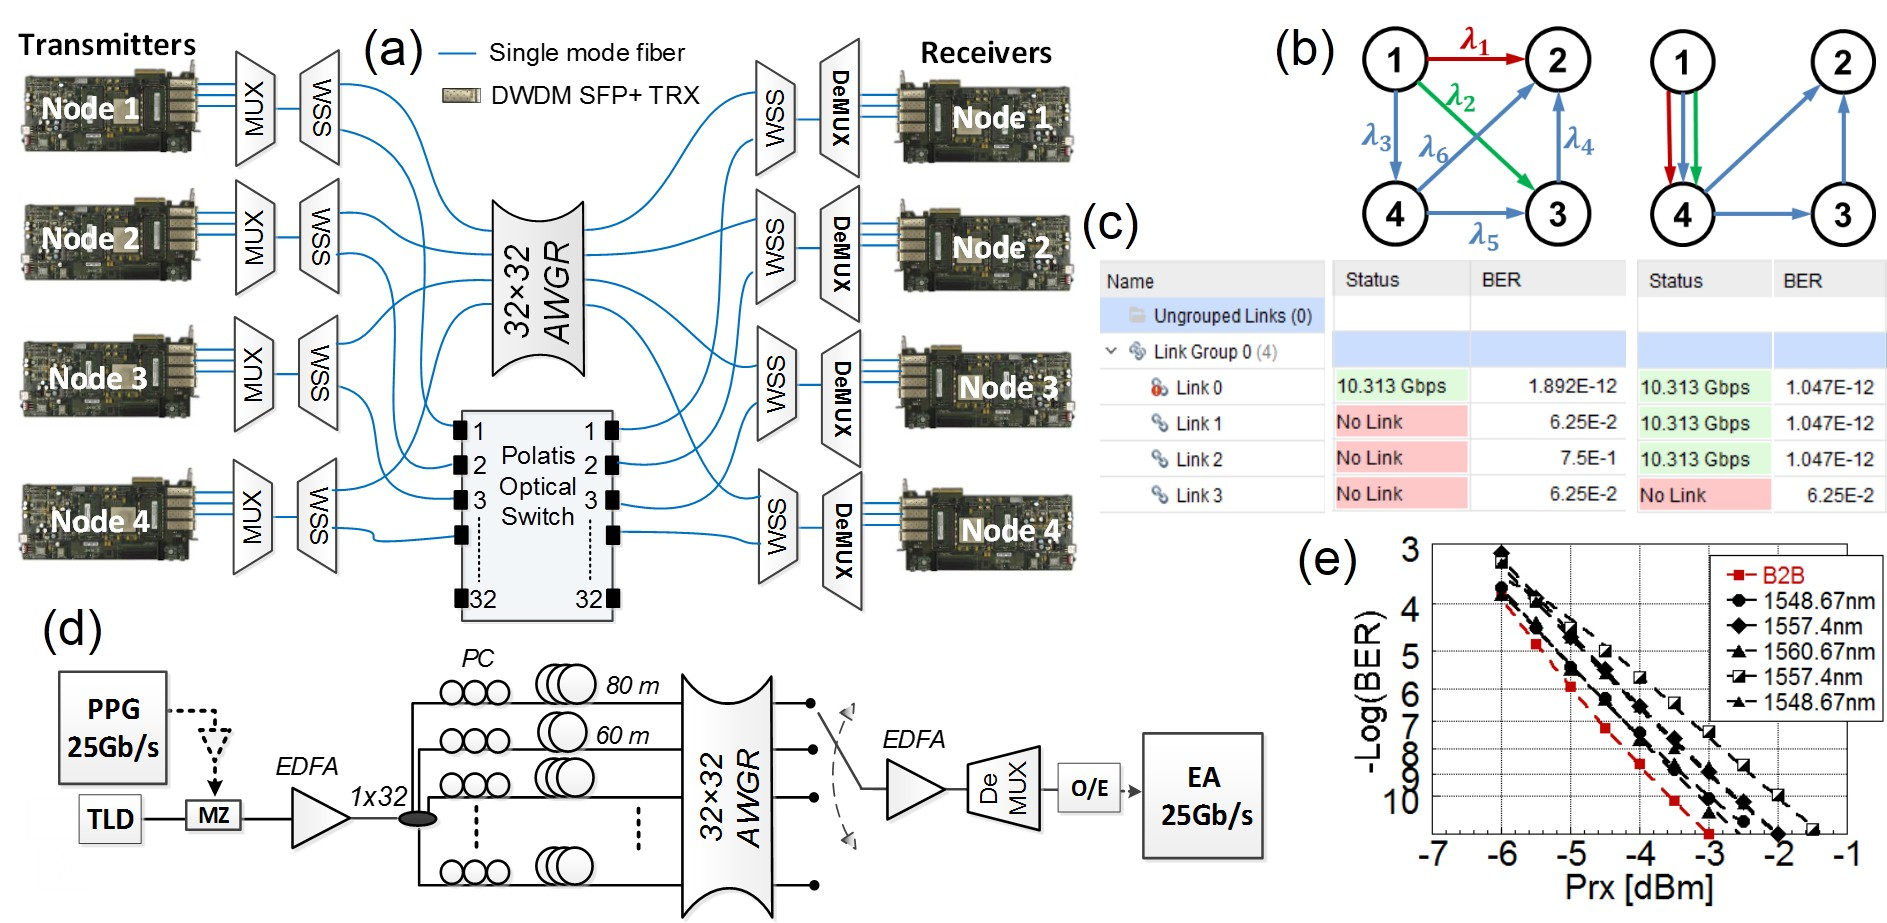
\includegraphics[width=15cm]{Figure2_v3.jpg}
\caption{(a) Four-node testbed to demonstrate the bandwidth steering principle. AWGR: arrayed waveguide grating router; Mux: multiplexer; Demux: demultiplexer; WSS: wavelength selective switch. (b) Connectivity before and after reconfiguration. (c) BER values at node4 before (one green link) and after reconfiguration (three green links). (d) Experiment setup for testing scalability to 32 nodes under worst-case crosstalk scenario (all-to-all). PPG: pulse pattern generator; EA: error analyzer; EDFA: erbium-doped fiber amplifier; PC: polarization controller; TLD: tunable laser diode; MZ: Mach Zehnder modulator. (e) BER measurements carried at 25 Gb/s per lambda in a 32-node all-to-all scenario under worst-case coherent crosstalk.}
\vspace{-3ex}
\end{figure}
Fig.2(d) shows the experiment setup we used to assess the physical layer scalability of the proposed system, which is mainly affected by the in-band crosstalk \cite{JOCN_ThinCLOS,AWGR_XT_1996}. The worst case condition is represented by the default all-to-all configuration, where each of the \textit{N} AWGR inputs would have have \textit{N} lambdas and each lambda at the AWGR outputs would have \textit{N}-1 in-band crosstalk components. Our experiment emulates this condition by using a 1$\times32$ power splitter to create 32 copies of the same signal (modulated at 25 Gb/s with On-Off Keying modulation) and sending each copy to a different AWGR input. The results in Fig.2(e) shows that the proposed system can achieve BER as low as 1E-12 with very low power penalty when using all the \textit{N}=32 ports of the AWGR used in Fig. 2(a) testbed. This means that the proposed system can support and aggregated bandwidth equal to 25 Gb/s$\times$32$\times$32$\times$2= 51.2 Tb/s. Future studies will investigate (1) FlexLION with larger port count (512 ports and beyond) using ThinCLOS AWGR \cite{JOCN_ThinCLOS} and (2) silicon photonic integration (SiPh) of the proposed system leveraging recent advances in SiPh AWGRs, microring filters and color-blind switches (e.g. \cite{Han:15, MZI-IBM}).  

%%\section{References}
%%References should be cited with the \verb+\cite{}+ command.
%%Bracketed citation style, as opposed to superscript, is preferred
%%\cite{vantrigt97,krishnan00,masters93,shoop97,kalman76,craig96,steup96}.
%%The \texttt{osameet3.sty} style file references \texttt{cite.sty}. Comprehensive journal abbreviations are available on the Crossref web site:
%%\href{http://www.crossref.org/titleList/}{http://www.crossref.org/titleList/}.
\bibliographystyle{IEEEtran}
{\footnotesize \bibliography{sample}}
%\section*{}
{\small \textit{This work was supported in part by DoD contract H98230-16-C-0820 and NSF grant 1611560.}\par}
%\footnote{test}
\end{document}
